\documentclass{article}

\usepackage{booktabs}
\usepackage{tabularx}
\usepackage{hyperref}
\usepackage[utf8]{inputenc}
\usepackage{graphicx}
\usepackage{lipsum}

\title{SE 3XA3: Development Plan\\The Resume Shotgun}

\author{Team 5, Proper Mars Tribe
		\\ Gavin Jameson, jamesong
		\\ Jeremy Langner, langnerj
		\\ Sam Gorman, gormans
}

\date{}

%\input{../Comments}

\begin{document}

\maketitle

\newpage

\tableofcontents

\newpage

This document outlines the group's initial plans for maintaining efficient and effective progress on the project as a collaborative effort.

\section{Team Meeting Plan}
The team will be meeting during regular weekly lab sections to plan and develop collaboratively. Outside of class time, the team will be using \href{https://lettucemeet.com/}{Lettuce Meet} to plan and schedule meeting times that work for everyone. From an initial assessment, Thursday and Friday nights will likely be the times allocated for any extra group work.

\section{Team Communication Plan}
Primary forms of communication will be through weekly lab sections and using a Discord group chat. The Discord group chat allows for text messaging, sharing files, sharing links, and unlimited voice calls.

\section{Team Member Roles}
A scribe will be designated for each significant team meeting, rotating between members each meeting. If a scribe can not attend a meeting, then the next group member will be chosen, with the original scribe taking up the role during the next meeting. It will be the role of the scribe to record what happens during meetings and update any plans accordingly. The order of rotation for scribes will be as follows: Jeremy Langner, Sam Gorman, Gavin Jameson.

Similarly, the team leader will rotate between meetings and be responsible for guiding and keeping meetings on track. The order of rotation for leaders will be as follows: Gavin Jameson, Jeremy Langner, Sam Gorman.

\section{Git Workflow Plan} \label{sec:gitflow}
The team plans on using a similar Git Workflow plan as presented in lecture  \href{https://nvie.com/posts/a-successful-git-branching-model/}{here}. This outline has two main branches with an infinite lifetime throughout the project - \textit{Master} and \textit{Develop}. The Master branch is used for main deliverables while the Develop branch is used for the incremental and developmental design process that yields frequent changes. Finally, each member will have their own individual branch to exclusively work independently on features and fixes that can be merged into Develop upon completion.

\section{Proof of Concept Demonstration Plan}
Our demonstration plan will consist of creating several non-existent students with random resumes with varying backgrounds. Once these are created, the next step is to use them to find compatible job matches with the application. During this demonstration however, there will not be a formal job application submission since these applicants do not exist. The function to actually apply will have to be demonstrated separately with a real applicant interested in the position. The part of the implementation plan that will be the most difficult is pulling the keywords from the sample resume to be used in comparison with the job application's keywords. The team will have to research potential APIs and other resources to use to make this task easier.

\section{Technology}
Since the original project is written in Python and it is a language that the team is comfortable using, the project will remain in Python. The supporting documentation will be generated with Doxygen as the team also has experience with it from previous classes. As mentioned in sections \ref{sec:gitflow} and \ref{sec:style}, the team will be following specific workflows and conventions - as Python has many capable IDEs, the team will use whichever is most comfortable that can maintain what was discussed in those sections. 

\section{Coding Style} \label{sec:style}
A few conventions will be followed:
\begin{itemize}
  \item Variables and functions will be named according to camel case, in which the first word begins with a lower case letter and all subsequent words are capitalized (ie. sumOfProducts()).
  \item Indentations will be achieved through four individual spaces rather than a \textbackslash tab character.
  \item Equations will be formatted with spaces in between numbers and operations, but not between numbers and brackets (ie. [1 + 2] ** 6 is proper form).
  \item Single line comments will be formatted with two comment characters, followed by a space, followed by the message (ie. \%\% Example Comment).
  \item Comments will be placed above important blocks of code, including but not limited to: Function declarations, variable initialization blocks, large loops or conditional statements, complicated mathematical equations. 
\end{itemize}

\section{Project Schedule}

\begin{figure}[htp]
    \centering
    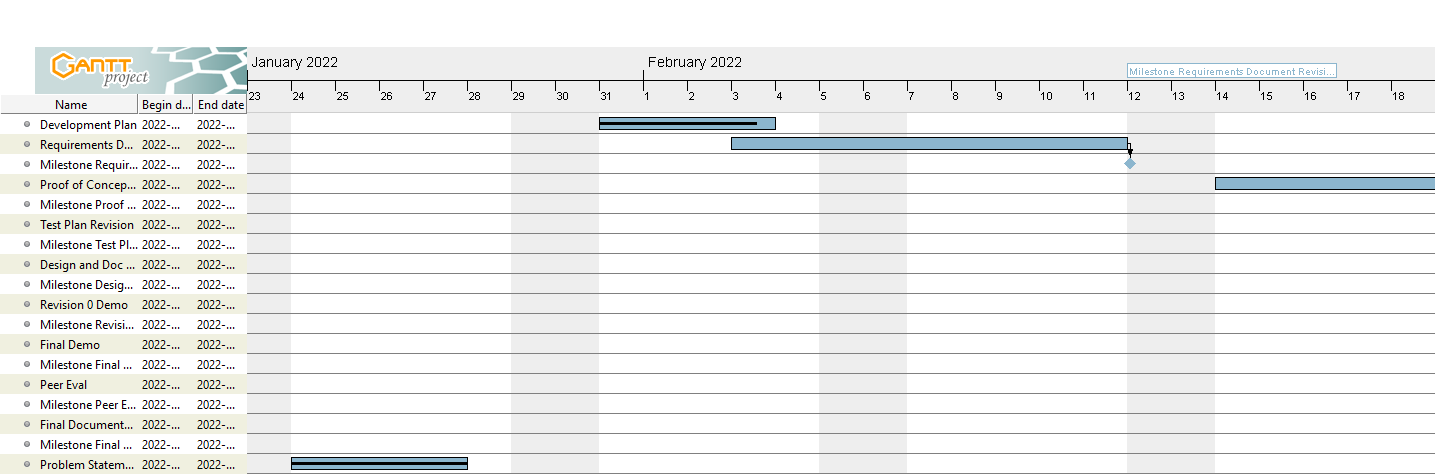
\includegraphics[width=\textwidth]{Gantt_Charts/3XA3_Gantt_1.png}
    \caption{Gantt Chart Jan 23 - Feb 19}
    \label{fig:gantt0}
\end{figure}

\begin{figure}[htp]
    \centering
    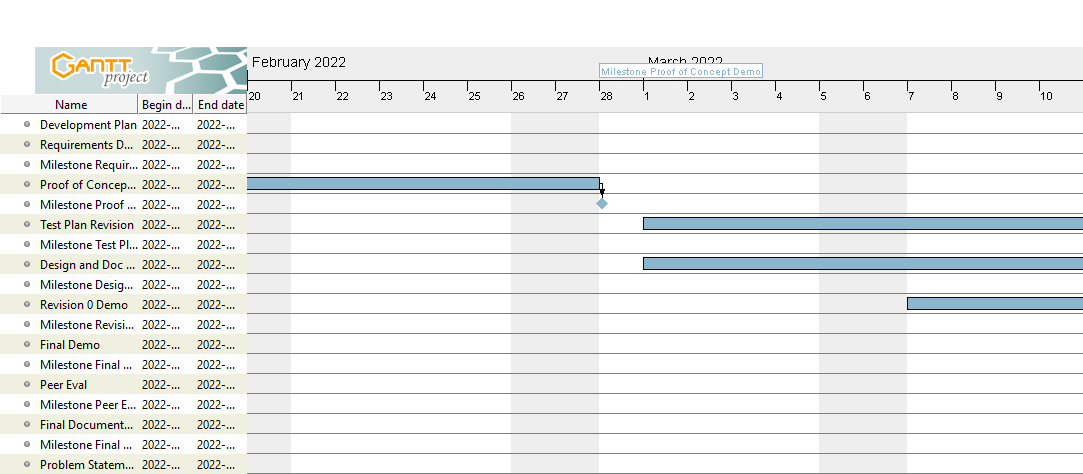
\includegraphics[width=\textwidth]{Gantt_Charts/3XA3_Gantt_2.png}
    \caption{Gantt Chart Feb 20 - March 11}
    \label{fig:gantt1}
\end{figure}

\begin{figure}[htp]
    \centering
    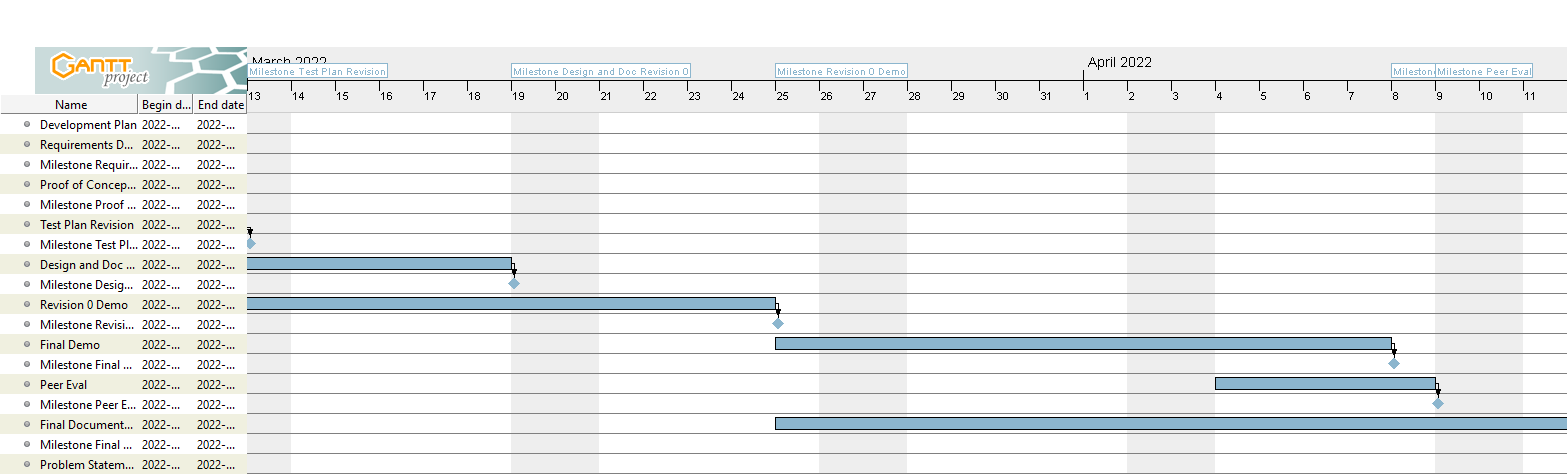
\includegraphics[width=\textwidth]{Gantt_Charts/3XA3_Gantt_3.png}
    \caption{Gantt Chart March 12 - April 12}
    \label{fig:gantt2}
\end{figure}

\begin{figure}[htp]
    \centering
    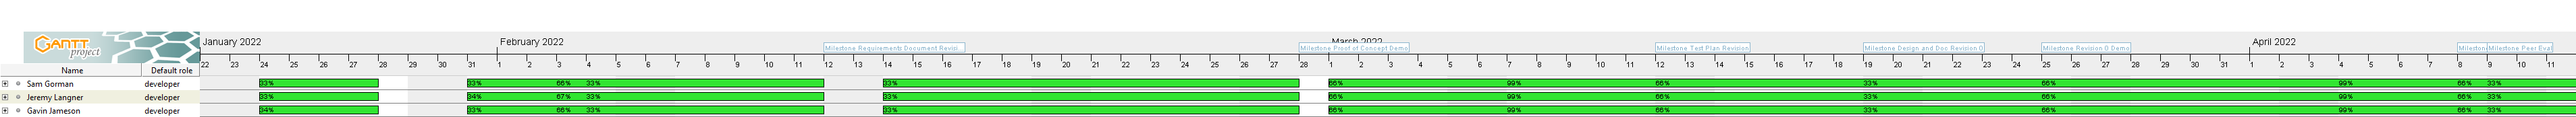
\includegraphics[width=\textwidth]{Gantt_Charts/3XA3_Gantt_Resources}
    \caption{Gantt Chart Resource Allocation} 
    \label{fig:gantt_resource}
\end{figure}

\clearpage

\section{Project Review}

There is currently nothing to review.

\newpage

\begin{table}[hp]
\caption{Revision History} \label{TblRevisionHistory}
\begin{tabularx}{\textwidth}{llX}
\toprule
\textbf{Date} & \textbf{Developer(s)} & \textbf{Change}\\
\midrule
February 1 & Everyone & Began out Team Meeting Plan, Team Communication Plan, Team Member Roles, Git Workflow Plan, Technology, and Coding Style. \\
February 3 & Everyone & Project Schedule, Revising previous sections\\ 
... & ... & ...\\
\bottomrule
\end{tabularx}
\end{table}

\end{document}